\subsubsection{Monitor}

La manera en que controlamos la ocupación de los espacios en el mapa, es decir, cómo evoluciona la trayectoria de cada robot es mediante el disparo de un Monitor implementado en Python. Este es el va a controlar, guiar y realizar la toma de decisiones para que cada robot pueda seguir su trayectoria sin interrumpir a los demás y por lo tanto no bloquear todo el sistema.

Para poder guiar a cada robot en su trayectoria, cada uno va a estar representado por un hilo lógico en el programa en Python. Más precisamente cuando existe un robot en el mundo real y se realiza el proceso de sincronización con el software, este va a crear un objeto (representación de un ente en la Programación Orientada a Objetos) el cual va a contener un conjunto de métodos implementados y entre ellos, la creación de un hilo en Python.

A su vez definimos cuál va a ser el punto de inicio y el punto final, es decir el comienzo del recorrido y el final del mismo, y el mapa es un modelo discreto representado por una Red de Petri. Podemos determinar cuales van a ser la plazas que el robot va a ocupar en un preciso momento y las transiciones que se van a disparar para que este pueda llegar a su destino. Con todos estos elementos le damos al monitor las herramientas para realizar su trabajo y efectuar los métodos que le permitan modificar el marcado de la Red de Petri.

\paragraph{Cola de cortesía} \mbox{} \vspace{8pt}

La manera en que el Monitor ejerce el control de la exclusión mutua dentro de la Red de Petri es mediante el uso de colas, entonces, cuando un hilo (robot) está dentro del monitor y aparece otro hilo que intenta ejecutar otro o el mismo procedimiento, el acceso al Monitor se bloquea e inserta el segundo hilo en una cola de cortesía usando una política FIFO. Cuando el primer hilo abandona el monitor, el segundo hilo (que se encuentra en el primer lugar de la cola) es el seleccionado por el Monitor para ejecutar sus tareas. Si la cola está vacía entonces el Monitor se encuentra libre y cualquier hilo que intente tomar el control de éste último podrá hacerlo sin intervención alguna.

\paragraph{Política del monitor} \mbox{} \vspace{8pt}

Así como mencionamos más arriba que hacemos uso de las colas del monitor para controlar la exclusión mutua, existe la posibilidad de que dos hilos (robots) intenten acceder a la misma plaza ya que su secuencia de disparos así lo determina. En ese caso vamos a tener que tomar una decisión de qué hilo es que va a lograr apoderarse de la plaza en primer lugar. Para esto hacemos uso de una Política definida por nosotros mismos, a partir de ella un hilo va a tener preferencia sobre otro. La política decide sobre todos los hilos que tengan una transición sensibilizada correspondiente a la celda que quiere ocupar.

Poniendo el caso en concreto de los robots que comparten un mapa, nos parece más acertada la idea de que un robot pueda terminar su recorrido de forma rápida y efectiva. Es por ello que cada robot va guardando el camino que va atravesando, es decir, las celdas por las cuales se desplazó y aumentando un contador interno. Este es el parámetro que se usa para determinar qué robot va a tener preferencia sobre otro, entonces, al momento de ocurrir un conflicto entre dos robots que intentan ocupar la misma celda, el Monitor va a evaluar que robot le falta menos camino por recorrer y va a elegirlo para ocupar el lugar en disputa. 

\paragraph{Solución de conflictos entre robots} \mbox{} \vspace{8pt}

Acá se representa el posible conflicto que puede ocurrir cuando dos robots intentan pasar por el mismo lugar (celda) ya que se su trayectoria así lo define. La figura \ref{fig:conflicto_map} muestra entonces que el robot A tiene como destino la celda $14$ mientras que el robot B tiene como destino la celda $16$ y la celda en conflicto es la $8$.

\begin{figure}[H]
    \centering
    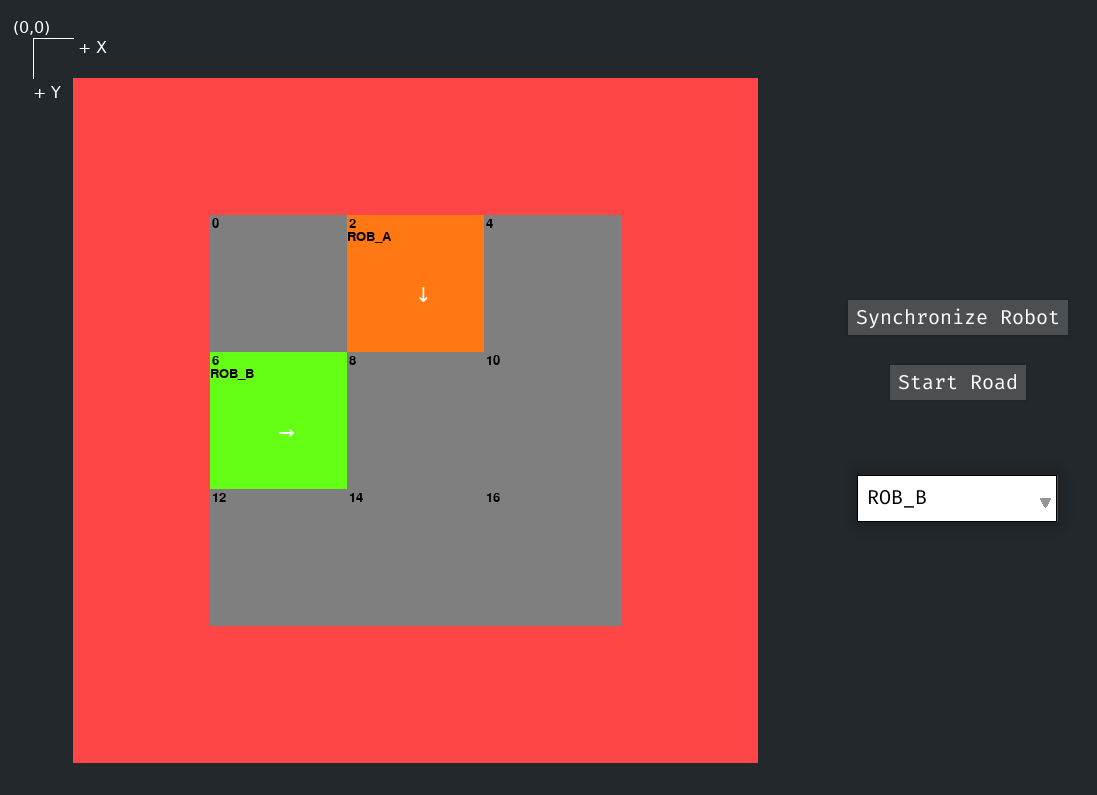
\includegraphics[trim={1.6cm 0.3cm 0 1.5cm}, clip, width=0.7\linewidth]{images/conflicto_map.png}
    \caption{Representación de un conflicto entre dos robots que intentan pasar por la misma celda}
    \label{fig:conflicto_map}
\end{figure}

Esta misma situación se la plantea en la figura \ref{fig:rdp_no_grid_conflicto} con una red de Petri con sus respectivos recursos que controlan la exclusión mutua de las celdas y las transiciones sensibilizadas marcadas en rojo $\{T_2, T_4, T_5, T_7, T_{11}, T_{13}\}$ que muestran los posibles caminos que puede tomar el robot dado el marcado actual de la red. El robot A intenta disparar la transición sensibilizada $T_7$ mientras que el robot B intenta hacer lo mismo pero con la transición $T_{11}$.

\begin{figure}[H]
    \centering
    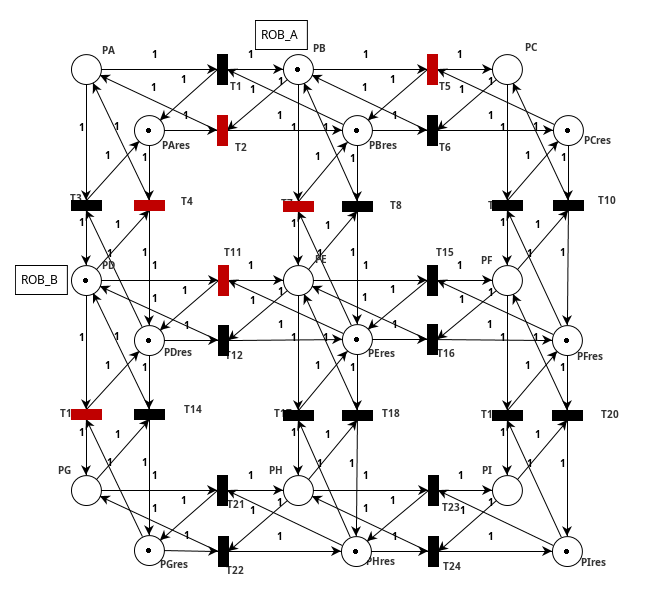
\includegraphics[width=0.8\linewidth]{images/rdp_no_grid_conflicto.png}
    \caption{Representación del conflicto de la figura \ref{fig:conflicto_map} en una red de Petri}
    \label{fig:rdp_no_grid_conflicto}
\end{figure}

El conflicto es resuelto mediante la política que se definió mas arriba en esta misma sub sección, y da como resolución que el robot A es el que avance en la ocupación de la celda en disputa tal como muestra la figura \ref{fig:conflicto_map_solucionado}. Esto significa que una vez que el robot A finalice su recorrido en la celda $14$, el robot B va a poder ocupar la celda $8$ y también terminar con su recorrido.

\begin{figure}[H]
    \centering
    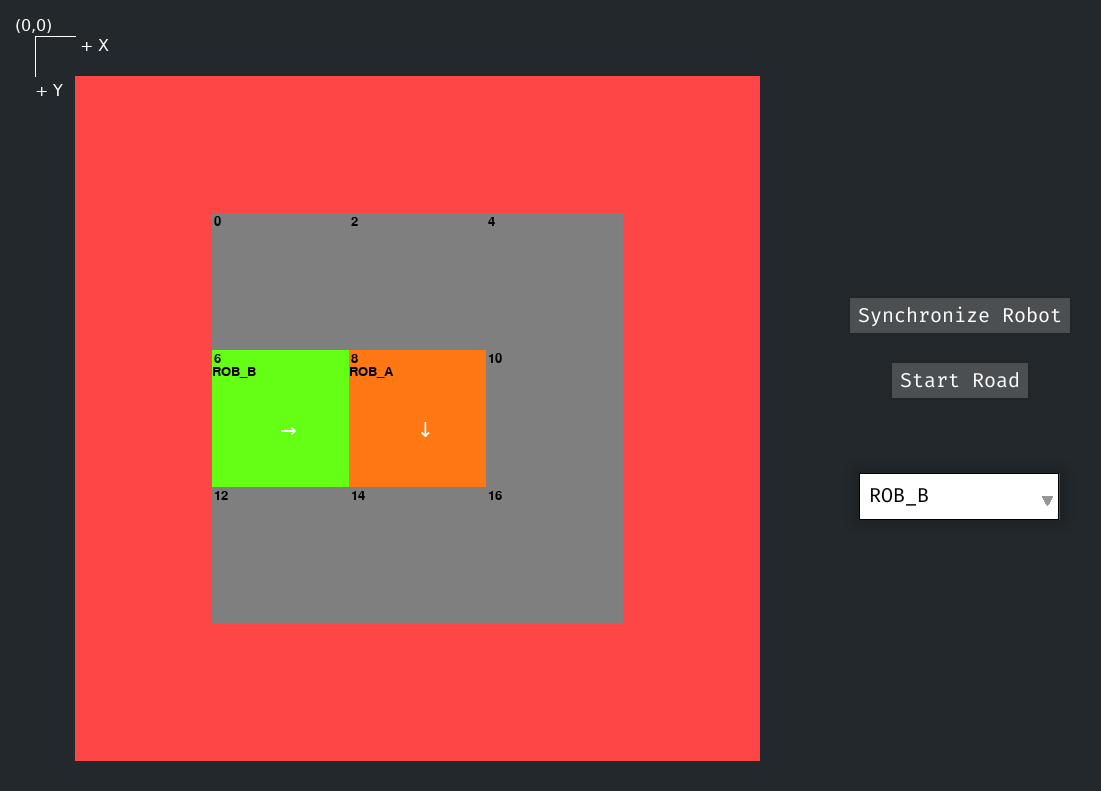
\includegraphics[trim={1.6cm 0.3cm 0 1.5cm}, clip, width=0.7\linewidth]{images/conflicto_map_solucionado.png}
    \caption{Resolución del conflicto de dos robots intentando pasar por la misma celda}
    \label{fig:conflicto_map_solucionado}
\end{figure}

La solución del conflicto también se ve representada en la red de Petri que muestra un marcado diferente en la figura \ref{fig:rdp_no_grid_conflicto_solucionado}, colocando al robot A en la plaza $PE$ y también revelando que las transiciones sensibilizas ahora son $\{T_4, T_8, T_{13}, T_{15}, T_{17}\}$ que por supuesto se diferencian al estar en color rojo. Ya resuelto el conflicto se puede observar que ahora el robot A tiene como posibilidad el disparo de la transición $T_{17}$ para llegar a su destino mientras que el robot B no puede avanzar hacia la plaza $PE$ porque se encuentra ocupada.

\begin{figure}[H]
    \centering
    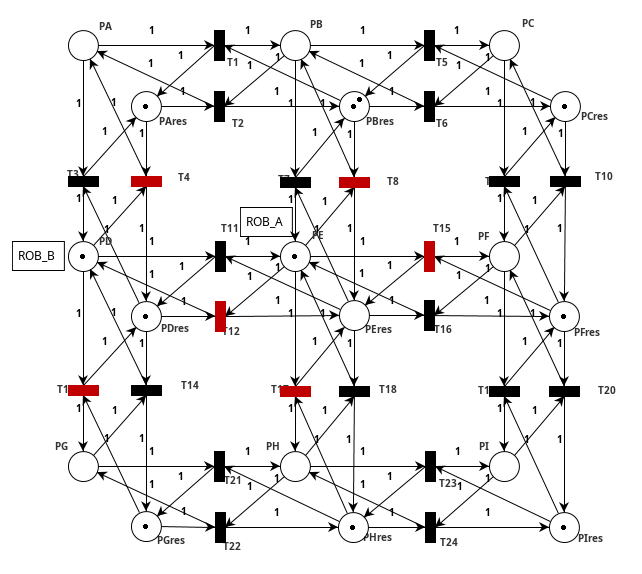
\includegraphics[width=0.8\linewidth]{images/rdp_no_grid_conflicto_solucionado.png}
    \caption{Resolución del conflicto entre los robots representado en una red de Petri y con el nuevo marcado de la red}
    \label{fig:rdp_no_grid_conflicto_solucionado}
\end{figure}

\paragraph{Funcionamiento del monitor} \mbox{} \vspace{8pt}

El funcionamiento del módulo del Monitor implementado en Python queda representado en el diagrama de secuencia de la figura \ref{fig:diagrama_monitor}.
Una de las cosas a tener en cuenta en el diagrama es que al Python estar limitado por la integración de $GIL$ y el manejo de los hilos, se vio la necesidad de implementar una condición para cada hilo en donde se le asigna una prioridad y por lo tanto el Monitor puede elegir cual va a ser el hilo a ejecutar. Esto se puede interpretar como la imposición sobre el mecanismo $GIL$ y forzarlo a elegir el hilo a ejecutar.

\begin{figure}[H]
    \centering
    \hspace*{-0,8cm}
    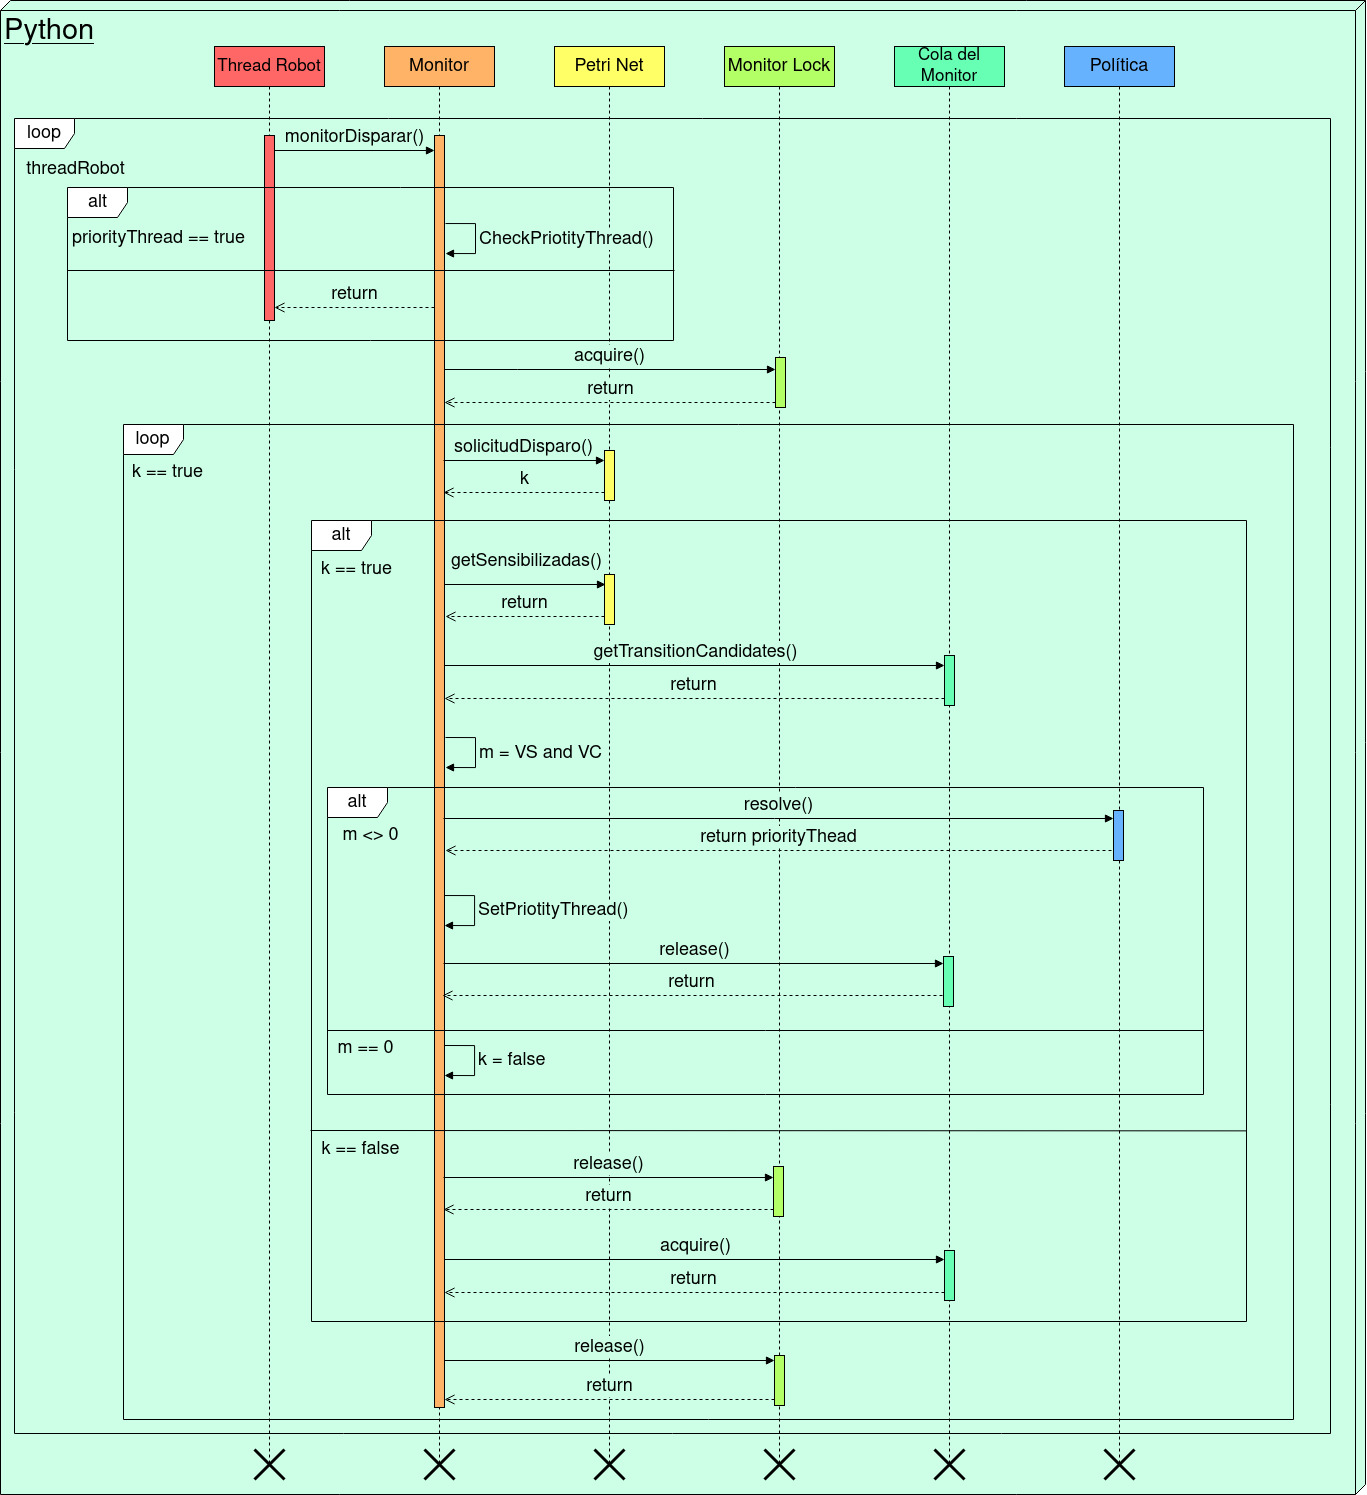
\includegraphics[width=1.2\linewidth]{images/diagrama_monitor.jpg}
    \caption{Diagrama de secuencia del monitor}
    \label{fig:diagrama_monitor}
\end{figure}

Puede darse la situación en que un hilo no dispare una transición ya que no cumple las condiciones para hacerlo. En este caso el hilo es agregado a la $Cola\ de\ hilos\ bloqueados$.

También puede surgir la situación en que dos robots entran en un conflicto donde pretenden intercambiar lugares, es decir que un robot intenta ocupar la celda del otro y viceversa cómo lo muestra la figura \ref{fig:conflicto_path}. Acá se ve involucrada la $Cola\ de\ hilos\ en\ conflicto$ donde se añaden los robots en cuestión. Este conflicto se soluciona mediante la implementación de una nueva política de re-calculo de trayectorias que toma como elementos de entrada la cola ya mencionada.

\begin{figure}[H]
    \centering
    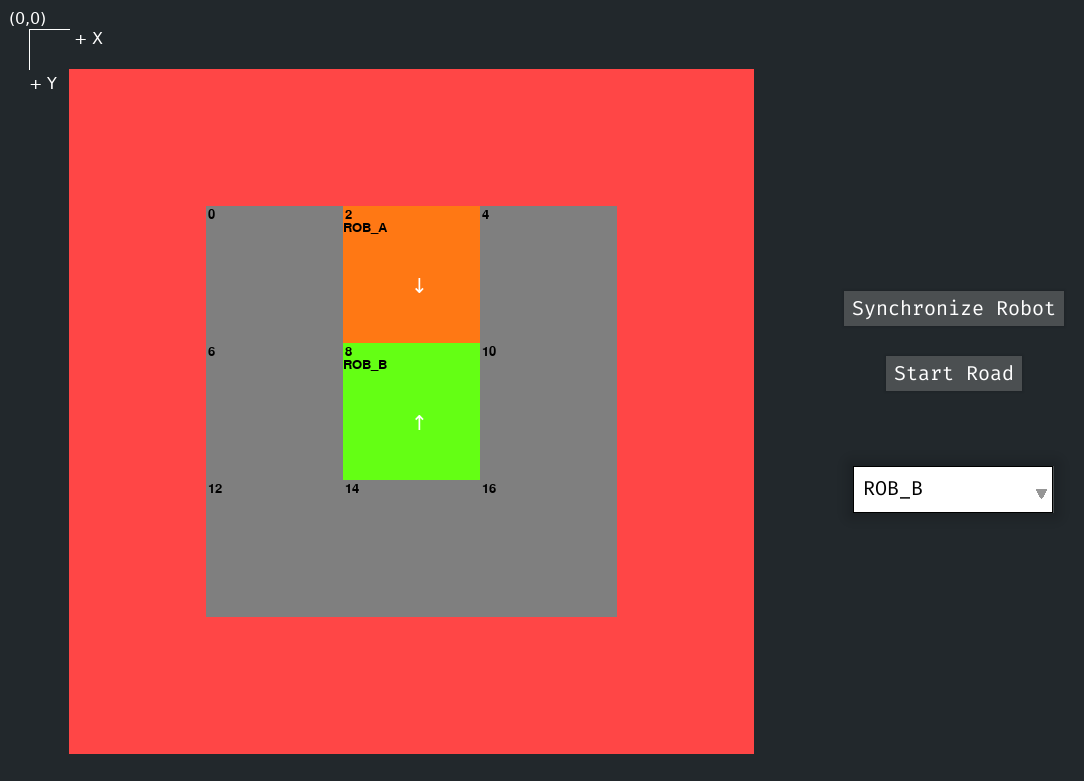
\includegraphics[trim={1.6cm 0.3cm 0 1.5cm}, clip, width=0.7\linewidth]{images/conflicto_path.png}
    \caption{Situación de conflicto en donde dos robots intentan intercambiar lugares}
    \label{fig:conflicto_path}
\end{figure}

Cabe destacar que el robot elegido por la política es penalizado dado que debe modificar su secuencia de coordenadas original (la más corta calculada por el algoritmo de $A*$) para darle lugar al otro robot. Esto implica que también se modifican las transiciones a disparar.

A continuación en la figura \ref{fig:diagrama_monitor_recalculate_path} se muestra en detalle la situación ya descrita y amplía el estado del Monitor cuando $k == false$ en el diagrama de secuencia \ref{fig:diagrama_monitor}.

\begin{figure}[H]
   \centering
   \hspace*{-2,0cm}
   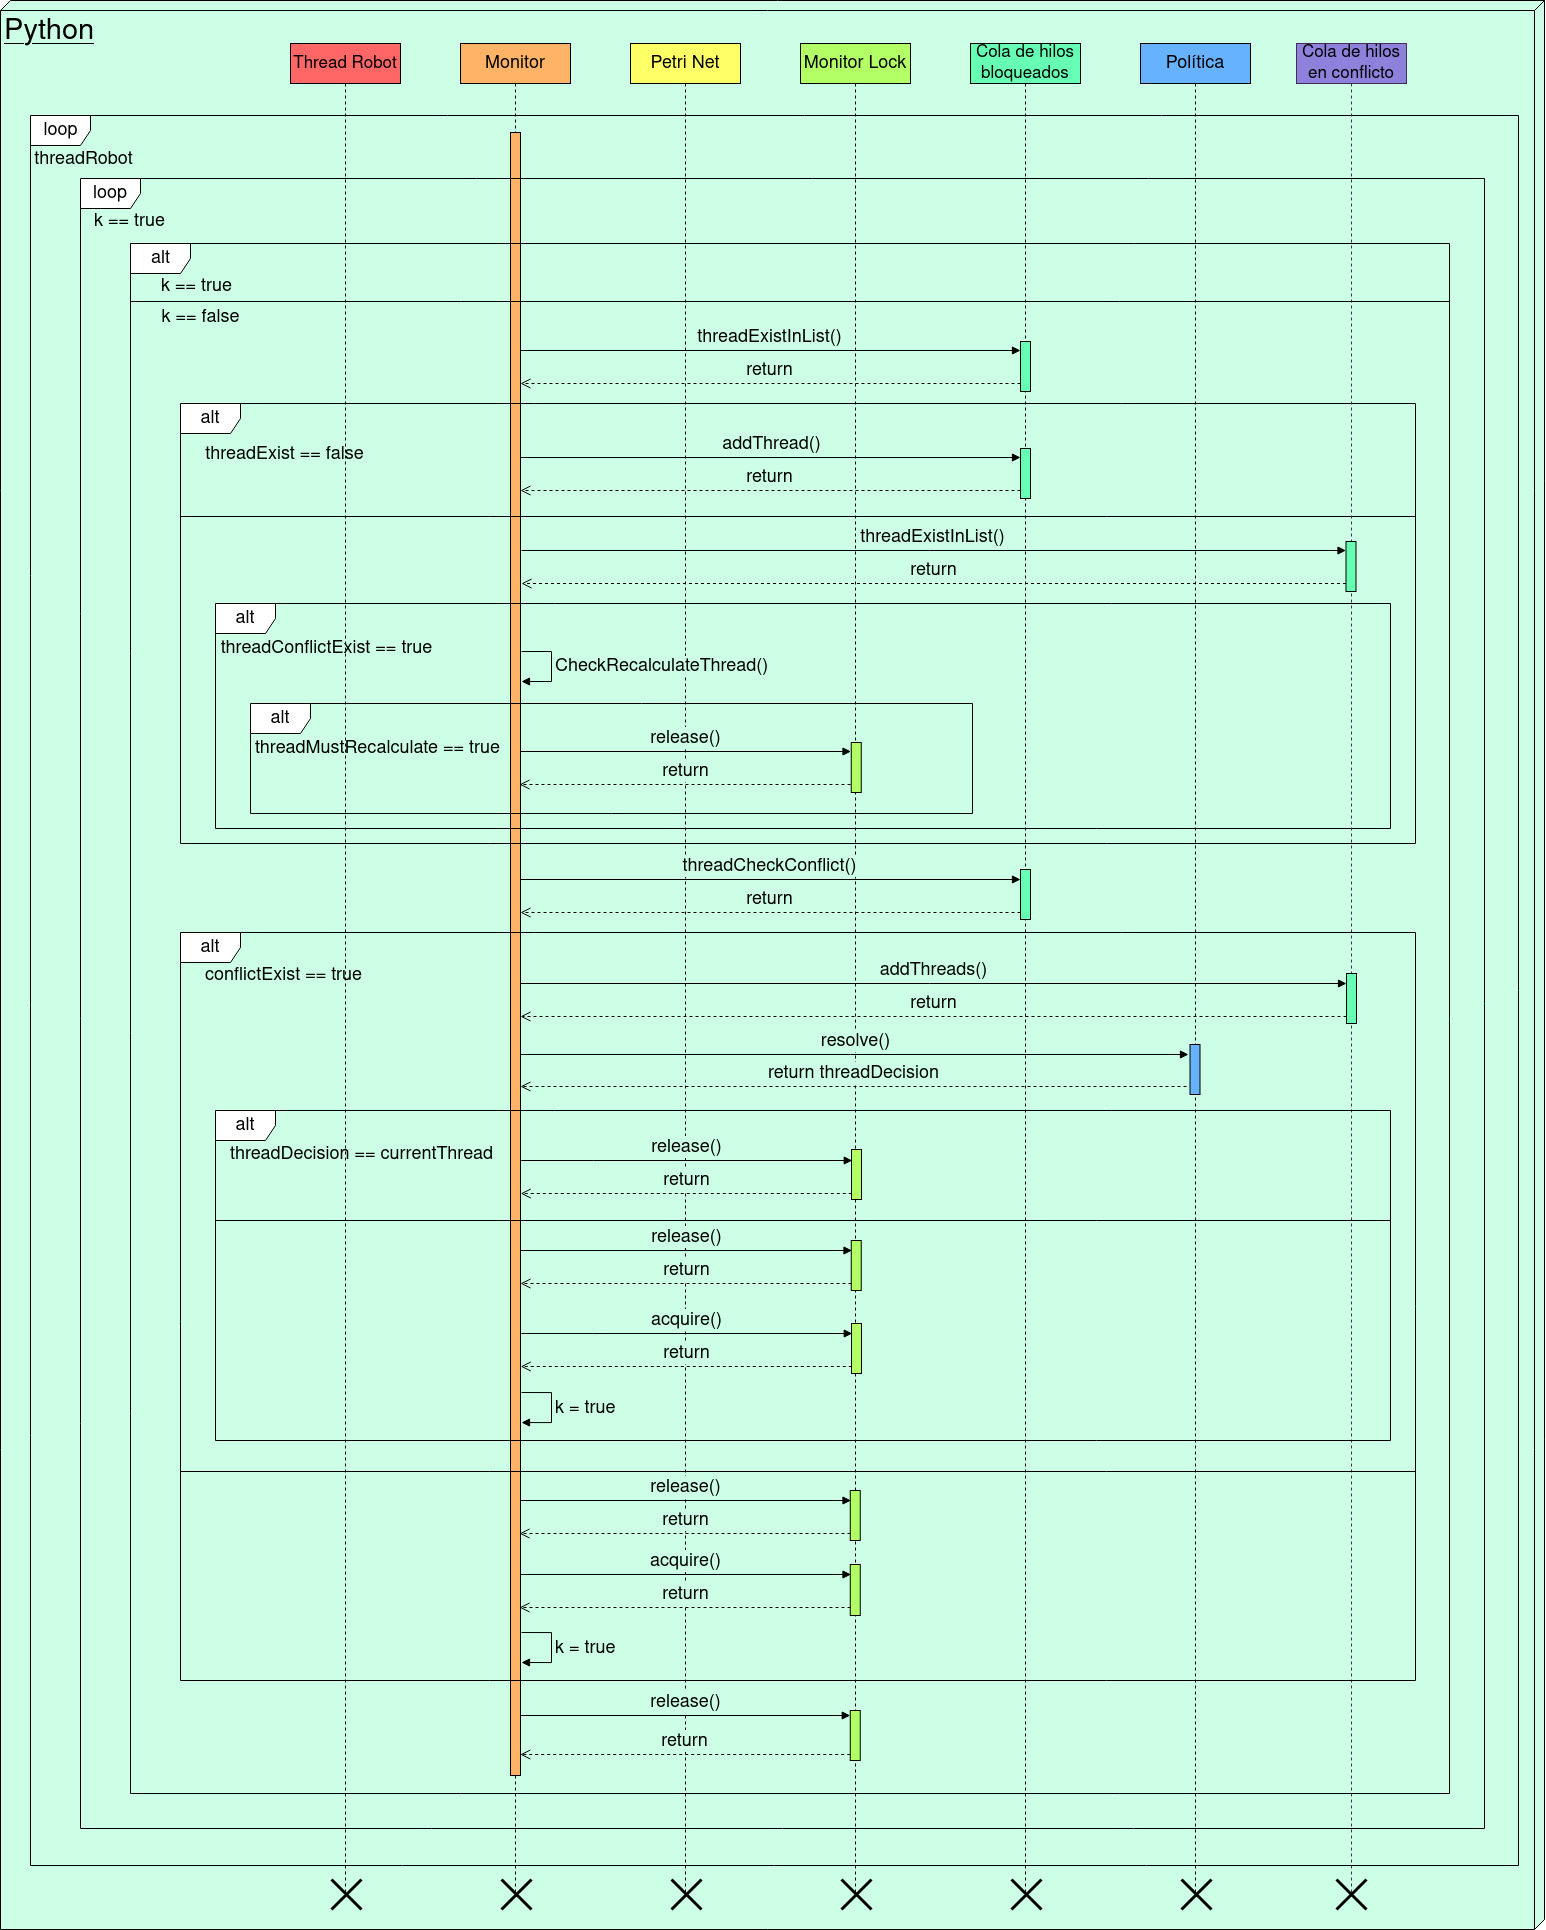
\includegraphics[width=1.3\linewidth]{images/diagrama_monitor_recalculate_path.jpg}
   \caption{Diagrama de secuencia del monitor que contempla la lógica de re-calcular la trayectoria de un robot bloqueado}
   \label{fig:diagrama_monitor_recalculate_path}
\end{figure}